%%%%%%%%%%%%%%%%%%%%%%%%%%%%%%%%%%%%%%%%%
% Masters/Doctoral Thesis 
% LaTeX Template
% Version 2.4 (22/11/16)
%
% This template has been downloaded from:
% http://www.LaTeXTemplates.com
%
% Version 2.x major modifications by:
% Vel (vel@latextemplates.com)
%
% This template is based on a template by:
% Steve Gunn (http://users.ecs.soton.ac.uk/srg/softwaretools/document/templates/)
% Sunil Patel (http://www.sunilpatel.co.uk/thesis-template/)
%
% Template license:
% CC BY-NC-SA 3.0 (http://creativecommons.org/licenses/by-nc-sa/3.0/)
%
%%%%%%%%%%%%%%%%%%%%%%%%%%%%%%%%%%%%%%%%%

%----------------------------------------------------------------------------------------
%	PACKAGES AND OTHER DOCUMENT CONFIGURATIONS
%----------------------------------------------------------------------------------------

\documentclass[
11pt, % The default document font size, options: 10pt, 11pt, 12pt
oneside, % Two side (alternating margins) for binding by default, uncomment to switch to one side
english, % ngerman for German
singlespacing, % Single line spacing, alternatives: onehalfspacing or doublespacing
%draft, % Uncomment to enable draft mode (no pictures, no links, overfull hboxes indicated)
%nolistspacing, % If the document is onehalfspacing or doublespacing, uncomment this to set spacing in lists to single
%liststotoc, % Uncomment to add the list of figures/tables/etc to the table of contents
%toctotoc, % Uncomment to add the main table of contents to the table of contents
%parskip, % Uncomment to add space between paragraphs
%nohyperref, % Uncomment to not load the hyperref package
headsepline, % Uncomment to get a line under the header
%chapterinoneline, % Uncomment to place the chapter title next to the number on one line
%consistentlayout, % Uncomment to change the layout of the declaration, abstract and acknowledgements pages to match the default layout
]{MastersDoctoralThesis} % The class file specifying the document structure

\usepackage[utf8]{inputenc} % Required for inputting international characters
\usepackage[T1]{fontenc} % Output font encoding for international characters
\usepackage{palatino} % Use the Palatino font by default

\usepackage[backend=bibtex,style=authoryear,natbib=true]{biblatex} % Use the bibtex backend with the authoryear citation style (which resembles APA)

\addbibresource{example.bib} % The filename of the bibliography

\usepackage[autostyle=true]{csquotes} % Required to generate language-dependent quotes in the bibliography

\usepackage{graphicx}
\usepackage{wrapfig}
\usepackage{lscape}
\usepackage{rotating}
\usepackage{epstopdf}

%\usepackage{hyperref}% http://ctan.org/pkg/hyperref
%\hypersetup{%
%  colorlinks = true,
%  linkcolor  = black
%}
%----------------------------------------------------------------------------------------
%	MARGIN SETTINGS
%----------------------------------------------------------------------------------------

\geometry{
	paper=a4paper, % Change to letterpaper for US letter
	inner=2.5cm, % Inner margin
	outer=3.8cm, % Outer margin
	bindingoffset=.5cm, % Binding offset
	top=1.5cm, % Top margin
	bottom=1.5cm, % Bottom margin
	%showframe, % Uncomment to show how the type block is set on the page
}

%----------------------------------------------------------------------------------------
%	THESIS INFORMATION
%----------------------------------------------------------------------------------------

\thesistitle{Testing of a micro service based application} % Your thesis title, this is used in the title and abstract, print it elsewhere with \ttitle
\supervisor{Giorgio \textsc{Malservisi}} % Your supervisor's name, this is used in the title page, print it elsewhere with \supname
\examiner{} % Your examiner's name, this is not currently used anywhere in the template, print it elsewhere with \examname
\degree{Software Quality Assurance postgraduate course} % Your degree name, this is used in the title page and abstract, print it elsewhere with \degreename
\author{Ferran \textsc{Montes}} % Your name, this is used in the title page and abstract, print it elsewhere with \authorname
\addresses{} % Your address, this is not currently used anywhere in the template, print it elsewhere with \addressname

\subject{IT and QA} % Your subject area, this is not currently used anywhere in the template, print it elsewhere with \subjectname
\keywords{} % Keywords for your thesis, this is not currently used anywhere in the template, print it elsewhere with \keywordnames
\university{\href{http://www.upc.edu}{Universitat Politècnica de Catalunya}} % Your university's name and URL, this is used in the title page and abstract, print it elsewhere with \univname
%\department{\href{https://www.fib.upc.edu}{FIB}} % Your department's name and URL, this is used in the title page and abstract, print it elsewhere with \deptname
%\group{\href{http://researchgroup.university.com}{Research Group Name}} % Your research group's name and URL, this is used in the title page, print it elsewhere with \groupname
%\faculty{\href{http://faculty.university.com}{Faculty Name}} % Your faculty's name and URL, this is used in the title page and abstract, print it elsewhere with \facname

\AtBeginDocument{
\hypersetup{pdftitle=\ttitle} % Set the PDF's title to your title
\hypersetup{pdfauthor=\authorname} % Set the PDF's author to your name
\hypersetup{pdfkeywords=\keywordnames} % Set the PDF's keywords to your keywords
}

\begin{document}

\frontmatter % Use roman page numbering style (i, ii, iii, iv...) for the pre-content pages

\pagestyle{plain} % Default to the plain heading style until the thesis style is called for the body content

%----------------------------------------------------------------------------------------
%	TITLE PAGE
%----------------------------------------------------------------------------------------

\begin{titlepage}
\begin{center}

\vspace*{.06\textheight}
{\scshape\LARGE \univname\par}\vspace{1.5cm} % University name
\textsc{\Large Postgraduate Report}\\[0.5cm] % Thesis type

\HRule \\[0.4cm] % Horizontal line
{\huge \bfseries \ttitle\par}\vspace{0.4cm} % Thesis title
\HRule \\[1.5cm] % Horizontal line
 
\begin{minipage}[t]{0.4\textwidth}
\begin{flushleft} \large
\emph{Author:}\\
\href{http://www.johnsmith.com}{\authorname} % Author name - remove the \href bracket to remove the link
\end{flushleft}
\end{minipage}
\begin{minipage}[t]{0.4\textwidth}
\begin{flushright} \large
\emph{Supervisor:} \\
\href{http://www.jamessmith.com}{\supname} % Supervisor name - remove the \href bracket to remove the link  
\end{flushright}
\end{minipage}\\[3cm]
 
\vfill

%\large \textit{A thesis submitted in fulfillment of the requirements\\ for the degree of \degreename}\\[0.3cm] % University requirement text
%\textit{in the}\\[0.4cm]
%\groupname\\\deptname\\[2cm] % Research group name and department name
 
\vfill

{\large \today}\\[4cm] % Date
%\includegraphics{Logo} % University/department logo - uncomment to place it
 
\vfill
\end{center}
\end{titlepage}

%----------------------------------------------------------------------------------------
%	DECLARATION PAGE
%----------------------------------------------------------------------------------------

%\begin{declaration}
%\addchaptertocentry{\authorshipname} % Add the declaration to the table of contents
%\noindent I, \authorname, declare that this thesis titled, \enquote{\ttitle} and the work presented in it are my own. I confirm that:

%\begin{itemize} 
%\item This work was done wholly or mainly while in candidature for a research degree at this University.
%\item Where any part of this thesis has previously been submitted for a degree or any other qualification at this University or any other institution, this has been clearly stated.
%\item Where I have consulted the published work of others, this is always clearly attributed.
%\item Where I have quoted from the work of others, the source is always given. With the exception of such quotations, this thesis is entirely my own work.
%\item I have acknowledged all main sources of help.
%\item Where the thesis is based on work done by myself jointly with others, I have made clear exactly what was done by others and what I have contributed myself.\\
%\end{itemize}
 
%\noindent Signed:\\
%\rule[0.5em]{25em}{0.5pt} % This prints a line for the signature
 
%\noindent Date:\\
%\rule[0.5em]{25em}{0.5pt} % This prints a line to write the date
%\end{declaration}

%\cleardoublepage

%----------------------------------------------------------------------------------------
%	QUOTATION PAGE
%----------------------------------------------------------------------------------------

%\vspace*{0.2\textheight}

%\noindent\enquote{\itshape Thanks to my solid academic training, today I can write hundreds of words on virtually any topic without possessing a shred of information, which is how I got a good job in journalism.}\bigbreak

%\hfill Dave Barry

%----------------------------------------------------------------------------------------
%	ABSTRACT PAGE
%----------------------------------------------------------------------------------------

\begin{abstract}
\addchaptertocentry{\abstractname} % Add the abstract to the table of contents
This project covers the test design and automated test implementation of a micro service based application simulating an e-commerce shop. Even though software development is not part of the focus of this course, in order to have a proper target for the set of tests defined, a small application based on the Spring framework is developed. The functionality of this application is specified through test cases written in Gherkin language and trying to simulate a Business Driven Development approach.
For test execution, the Java implementation of the Cucumber framework has been used. At the same time, automation is achieved through a Jenkins pipeline putting more emphasis in environment administration with Docker.
\end{abstract}

%----------------------------------------------------------------------------------------
%	ACKNOWLEDGEMENTS
%----------------------------------------------------------------------------------------

%\begin{acknowledgements}
%\addchaptertocentry{\acknowledgementname} % Add the acknowledgements to the table of contents
%The acknowledgments and the people to thank go here, don't forget to include your project advisor\ldots
%\end{acknowledgements}

%----------------------------------------------------------------------------------------
%	LIST OF CONTENTS/FIGURES/TABLES PAGES
%----------------------------------------------------------------------------------------

\hypersetup{linkcolor=black}
\tableofcontents % Prints the main table of contents

\listoffigures % Prints the list of figures

\listoftables % Prints the list of tables

%----------------------------------------------------------------------------------------
%	ABBREVIATIONS
%----------------------------------------------------------------------------------------

\begin{abbreviations}{ll} % Include a list of abbreviations (a table of two columns)

\textbf{SQA} & \textbf{S}oftware \textbf{Q}uality \textbf{A}ssurance\\
\textbf{BDD} & \textbf{B}usiness \textbf{D}riven \textbf{D}evelopment\\
\textbf{PoC} & \textbf{P}roof \textbf{o}f \textbf{C}oncept\\
\textbf{UI} & \textbf{U}ser \textbf{I}nterface\\
\textbf{REST} & \textbf{RE}presentational \textbf{S}tate \textbf{T}ransfer\\
\textbf{API} & \textbf{A}pplication \textbf{P}rogramming \textbf{I}interface\\



\end{abbreviations}

%----------------------------------------------------------------------------------------
%	PHYSICAL CONSTANTS/OTHER DEFINITIONS
%----------------------------------------------------------------------------------------

%\begin{constants}{lr@{${}={}$}l} % The list of physical constants is a three column table

% The \SI{}{} command is provided by the siunitx package, see its documentation for instructions on how to use it

%Speed of Light & $c_{0}$ & \SI{2.99792458e8}{\meter\per\second} (exact)\\
%Constant Name & $Symbol$ & $Constant Value$ with units\\

%\end{constants}

%----------------------------------------------------------------------------------------
%	SYMBOLS
%----------------------------------------------------------------------------------------

%\begin{symbols}{lll} % Include a list of Symbols (a three column table)

%$a$ & distance & \si{\meter} \\
%$P$ & power & \si{\watt} (\si{\joule\per\second}) \\
%Symbol & Name & Unit \\

%\addlinespace % Gap to separate the Roman symbols from the Greek

%$\omega$ & angular frequency & \si{\radian} \\

%\end{symbols}

%----------------------------------------------------------------------------------------
%	DEDICATION
%----------------------------------------------------------------------------------------

%\dedicatory{For/Dedicated to/To my\ldots} 

%----------------------------------------------------------------------------------------
%	THESIS CONTENT - CHAPTERS
%----------------------------------------------------------------------------------------

\mainmatter % Begin numeric (1,2,3...) page numbering

\pagestyle{thesis} % Return the page headers back to the "thesis" style

% Include the chapters of the thesis as separate files from the Chapters folder
% Uncomment the lines as you write the chapters

% Chapter 1

\chapter{The Application} % Main chapter title

\label{Chapter1} % For referencing the chapter elsewhere, use \ref{Chapter1} 

%----------------------------------------------------------------------------------------

% Define some commands to keep the formatting separated from the content 
\newcommand{\keyword}[1]{\textbf{#1}}
\newcommand{\tabhead}[1]{\textbf{#1}}
\newcommand{\code}[1]{\texttt{#1}}
\newcommand{\file}[1]{\texttt{\bfseries#1}}
\newcommand{\option}[1]{\texttt{\itshape#1}}

%----------------------------------------------------------------------------------------

\section{Overview}
The application consists on 6 services simulating an e-commerce application.

\begin{figure}
\centering
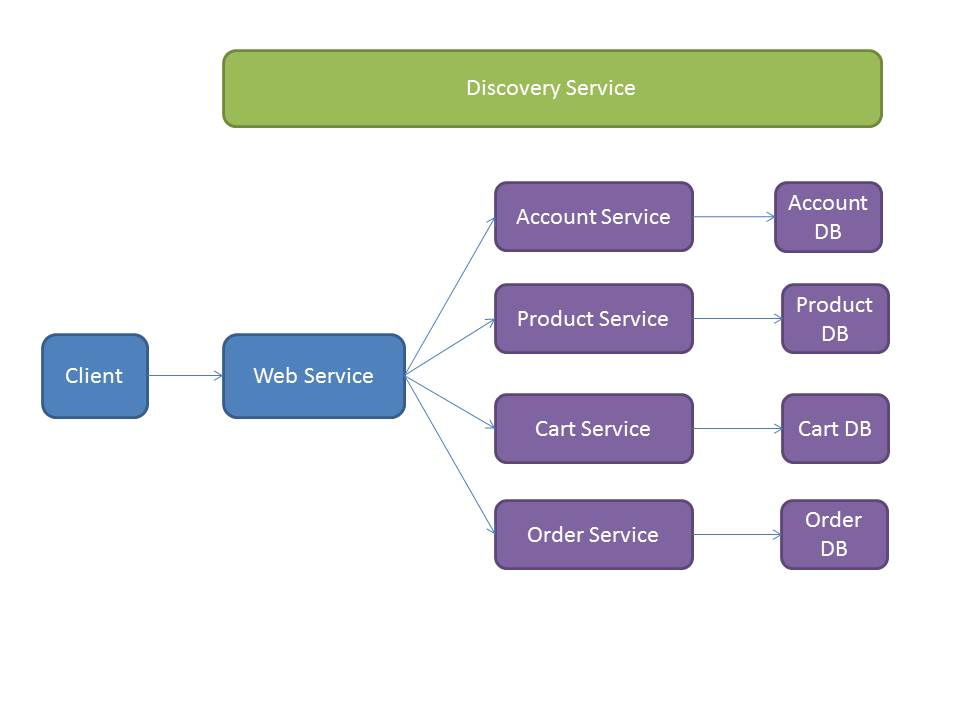
\includegraphics[width=\textwidth,height=\textheight,keepaspectratio]{Figures/Presentation1}
\decoRule
\caption[Block Diagram]{Application block diagram}
\label{fig:Block Diagram}
\end{figure}

The user entry point is the Web Service, from where all the functionality of the application can be accessed. For the sake of simplicity there are no roles defined within the users of the application and thus any request coming from the Web Service is processed by the application.
The Discovery Service is not focussed on functional requirements but it tracks all the available instances of each running service.

What follows is a short description of each one of the services:
\begin{itemize}
\item Web Service: User entry point. Application's functionality is accessed through a REST API 
\item Account Service: Service for managing user accounts. Accounts can be created and deleted.
\item Product Servive: Service that manages the shop product catalogue. Products can be created and deleted.
\item Cart Service: Service that manages the products within the shopping carts.
\item Order Service: Service that manages the carts within the shopping orders.
\item Discovery Service: Discussion of the experimental results
\end{itemize}

Relationships between services as well as the own service behavior is described within the test specification itself and so more details can be found in the next chapter. 

%----------------------------------------------------------------------------------------

\section{Data Model}

The Accounts, Product, Cart and Order Services have each one its own data model:
TODO: Data model classes

%----------------------------------------------------------------------------------------

\section{Assumptions}

All databases start with one test entry:

\begin{itemize}
\item Account: 000000001, "TestUser", 1000
\item Product: ref001, "10", "Simple mouse"
\item Cart: C001, 000000001, ref001
\item Order: O001, C001
\end{itemize}
 %Introduction and Objectives;
% Chapter 2

\chapter{The Application} % Main chapter title

\label{Chapter2} % For referencing the chapter elsewhere, use \ref{Chapter1} 

%----------------------------------------------------------------------------------------

% Define some commands to keep the formatting separated from the content 
%\newcommand{\keyword}[1]{\textbf{#1}}
%\newcommand{\tabhead}[1]{\textbf{#1}}
%\newcommand{\code}[1]{\texttt{#1}}
%\newcommand{\file}[1]{\texttt{\bfseries#1}}
%\newcommand{\option}[1]{\texttt{\itshape#1}}

%----------------------------------------------------------------------------------------

\section{Overview}
\paragraph In this chapter the application under test is described at high level and should be considered an introduction to \ref{Chapter3} where the application is described in greater detail but from the BDD point of view. As the development does not start from scratch but from a micro service Sprint demo, this chapter also describes what is already done and the improvements to be done during Project development based on BDD.

\paragraph The application consists on 6 services simulating an e-commerce application. A block diagram representation of the whole system is represented in figure \ref{fig:Block Diagram}.

\begin{figure}
\centering
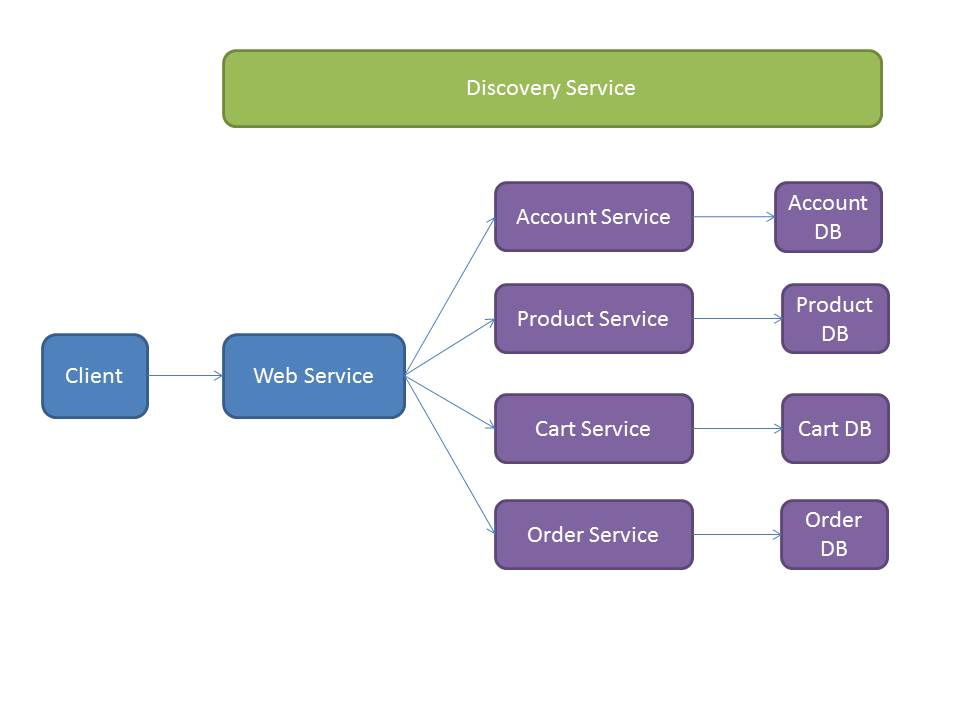
\includegraphics[width=\textwidth,height=\textheight,keepaspectratio]{Figures/Presentation1}
\decoRule
\caption[Block Diagram]{Application block diagram}
\label{fig:Block Diagram}
\end{figure}

\paragraph The user entry point is the Web Service, from where all the functionality of the application can be accessed. For the sake of simplicity there are no roles defined within the users of the application and thus any request coming from the Web Service is processed by the application.
There is no stock data either, considering that there is an unlimited amount available of each product added to the catalog represented by the Product Service database.
The Discovery Service is not focused on functional requirements but it tracks all the available instances of each running service.

\paragraph What follows is a short description of each one of the services:
\begin{itemize}
\item Web Service: User entry point. Application's functionality is accessed by the user through a UI provided by this service.
\item Account Service: Service for managing user accounts. Accounts can be created and deleted.
\item Product Service: Service that manages the shop product catalog. Products can be created and deleted.
\item Cart Service: Service that manages the products within the shopping carts.
\item Order Service: Service that manages the carts within the shopping orders.
\item Discovery Service: Service that manages the open instances of each one of the other services.
\end{itemize}

\paragraph Each one of the service implements and maintains its own relational database, without any link with other service's databases. Those services that need information from other services get it from the user through the Web Service. This means that the REST API exposed by all services consists at least on both "get" and "set" requests in order to be able to pull and push information from and to the system.
 
\paragraph Application behavior is shaped with the Gherkin files written for testing the services trying to simulate a BDD approach. More details on this follow in the next chapter. 

%----------------------------------------------------------------------------------------

\section{Data Model}

The Accounts, Product, Cart and Order Services have each one its own data model:\\


\textbf{Account Service}
\begin{itemize}
\item Number: int
\item Owner: string
\item Balance: float\\
\end{itemize}


\textbf{Product Service}
\begin{itemize}
\item Reference: string
\item Price: float
\item Description: string\\
\end{itemize}


\textbf{Cart Service}
\begin{itemize}
\item Name: string
\item AssociatedAccount: Account
\item AssociatedProducts: Product[]\\
\end{itemize}


\textbf{Order Service}
\begin{itemize}
\item Id: string
\item AssociatedCart: Cart\\
\end{itemize}

%----------------------------------------------------------------------------------------

\section{Technological Stack}
This application makes use of the following, third party, open source libraries:

\begin{itemize}
\item Programming language: Java JDK v1.8
\item Build tool: Apache Maven 3.3.9
\item Spring Framework Brixton Release: Spring Boot, Spring Cloud, Spring Data
\item Data Base: HyperSQL
\item Test execution FW: JUnit 4.11
\item Gherkin interpreter: cucumber-java 1.1.8
\item Docker Engine: 1.12.6
\end{itemize}


\section{Configuration}
The application is packaged within a single JAR file with all the services and the test framework with the Cucumber libraries and the implementation of the test steps for test execution. Having developed all services in one single project and thus using one single package certainly does not follow the philosophy of using micro services as it makes This simplifies showing how the application works. Each one of the services exposes a different port

\begin{itemize}
\item Web Service: 				localhost:1111
\item Account Service: 		localhost:2222
\item Product Service: 		localhost:3333
\item Order Service: 			localhost:4444
\item Cart Service: 			localhost:5555
\item Discovery Service: 	localhost:6666
\end{itemize}


\section{Assumptions}
Some assumptions and restrictions have been done when programming the application mainly to ease the coding part of the application, which actually is not a topic included in the course agenda.\\
 
- There are no user roles within the application. Any user can both create products and accounts as well as create carts and buy products through orders. This makes no sense from the functional point of view but eases the programming of the application.\\

- No stock data is used. Offering the possibility of increase and decrease the product stocks would create some relationships between services and their databases that would have added complexity to the coding.\\

- All databases are initialized with one test entry:

\begin{itemize}
\item Account: 000000001, "TestUser", 1000
\item Product: ref001, "10", "Simple mouse"
\item Cart: C001, 000000001, ref001
\item Order: O001, C001
\end{itemize}
 %Application
% Chapter 3

\chapter{Test Specification} % Main chapter title

\label{Chapter3} % For referencing the chapter elsewhere, use \ref{Chapter1} 

%----------------------------------------------------------------------------------------

% Define some commands to keep the formatting separated from the content 
%\newcommand{\keyword}[1]{\textbf{#1}}
%\newcommand{\tabhead}[1]{\textbf{#1}}
%\newcommand{\code}[1]{\texttt{#1}}
%\newcommand{\file}[1]{\texttt{\bfseries#1}}
%\newcommand{\option}[1]{\texttt{\itshape#1}}

%----------------------------------------------------------------------------------------

\section{Overview}
\paragraph The test specification explained in this chapter serve also as a driver for the application design and development. While in the previous chapter was described the data model of each one of the services that form the application, in this one the behavior of each component as well as its connections with other services are explained through a set of Gherkin based files scoped at different test levels. The intention is  to simulate a BDD process and thus the test design process is the following:

\begin{enumerate}
	\item For each test level, define a Gherkin file that describes a functionality
	\item That file is then reviewed by the related stakeholders
	\item The functionality that will make that test set to pass is implemented
\end{enumerate}

\paragraph Of course item 2 is not happening during the implementation of this Project but is good to mention it anyway as it is quite the essence of using Gherkin language for test specification. The using of plain English files for describing how an application works should allow any stakeholder to participate openly in the way software is designed achieving greater team integration, improving communication and reducing misunderstandings to a minimum. Although its difficult to reflect the simulation of the BDD process in this document, the author will try to go through items 1 and 3 of the process in order to get an introduction as reliable as possible of an actual BDD process.

%\paragraph The reason behind using the process listed above is actually to compare previous test design strategies used by the author with this approach in a more complex application than the one used in the course. So the decision of using BDD instead of other strategies is just the auto imposed constraint of including it as one of the Project objectives and not the result of a comparison between different strategies.


%----------------------------------------------------------------------------------------

\section{Features}
\paragraph From the functional point of view, there have been defined two test levels for covering the major part of the use cases for the application:

\begin{itemize}
\item Integration Level: covers test cases coming from the integration of the Web Service and each one of the other services.
\item System Level: covers test cases that need the whole system to work. This is, use cases where interaction with different services is needed.
\end{itemize}

\paragraph From the non functional point of view, only test cases regarding availability have been considered. Test cases here involve the Discovery service and its ability to manage instances of the functional services.

\paragraph The following sub sections have been named after the feature file names, and in it is auto included the test type (either functional or non functional), the test level (either integration or system level), the service involved, and the test case number.

\subsection{functional-it-accountservice-1}
\ttfamily
\begingroup
\obeylines
\input{./../../sqa-project/features/functional-it-accountservice-1.feature}%
\endgroup%

\subsection{functional-it-accountservice-2}
\begingroup
\obeylines
\input{./../../sqa-project/features/functional-it-accountservice-2.feature}%
\endgroup%

\subsection{functional-it-accountservice-3}
\begingroup
\obeylines
\input{./../../sqa-project/features/functional-it-accountservice-3.feature}%
\endgroup%

\subsection{functional-it-productservice-1}
\begingroup
\obeylines
\input{./../../sqa-project/features/functional-it-productservice-1.feature}%
\endgroup%

\subsection{functional-it-orderservice-1}
\begingroup
\obeylines
\input{./../../sqa-project/features/functional-it-orderservice-1.feature}%
\endgroup%

\subsection{functional-it-cartservice-1}
\begingroup
\obeylines
\input{./../../sqa-project/features/functional-it-cartservice-1.feature}%
\endgroup%

\subsection{functional-st-1}
\begingroup
\obeylines
\input{./../../sqa-project/features/functional-st-1.feature}%
\endgroup%

\subsection{functional-st-2}
\begingroup
\obeylines
\input{./../../sqa-project/features/functional-st-2.feature}%
\endgroup%

\subsection{nonfunctional-availability-accounts}
\begingroup
\obeylines
\input{./../../sqa-project/features/nonfunctional-availability-accounts.feature}%
\endgroup%

\subsection{nonfunctional-availability-product}
\begingroup
\obeylines
\input{./../../sqa-project/features/nonfunctional-availability-product.feature}%
\endgroup%

\subsection{nonfunctional-availability-cart}
\begingroup
\obeylines
\input{./../../sqa-project/features/nonfunctional-availability-cart.feature}%
\endgroup%

\subsection{nonfunctional-availability-order}
\begingroup
\obeylines
\input{./../../sqa-project/features/nonfunctional-availability-order.feature}%
\endgroup%
\normalfont

\section{Class Diagram}
\paragraph After describing the application requirements in the previous sub chapters, the main relationships and dependencies between services are set. The diagram \ref{fig:Class Diagram} shows those dependencies.

\begin{figure}[!htb]
\centering
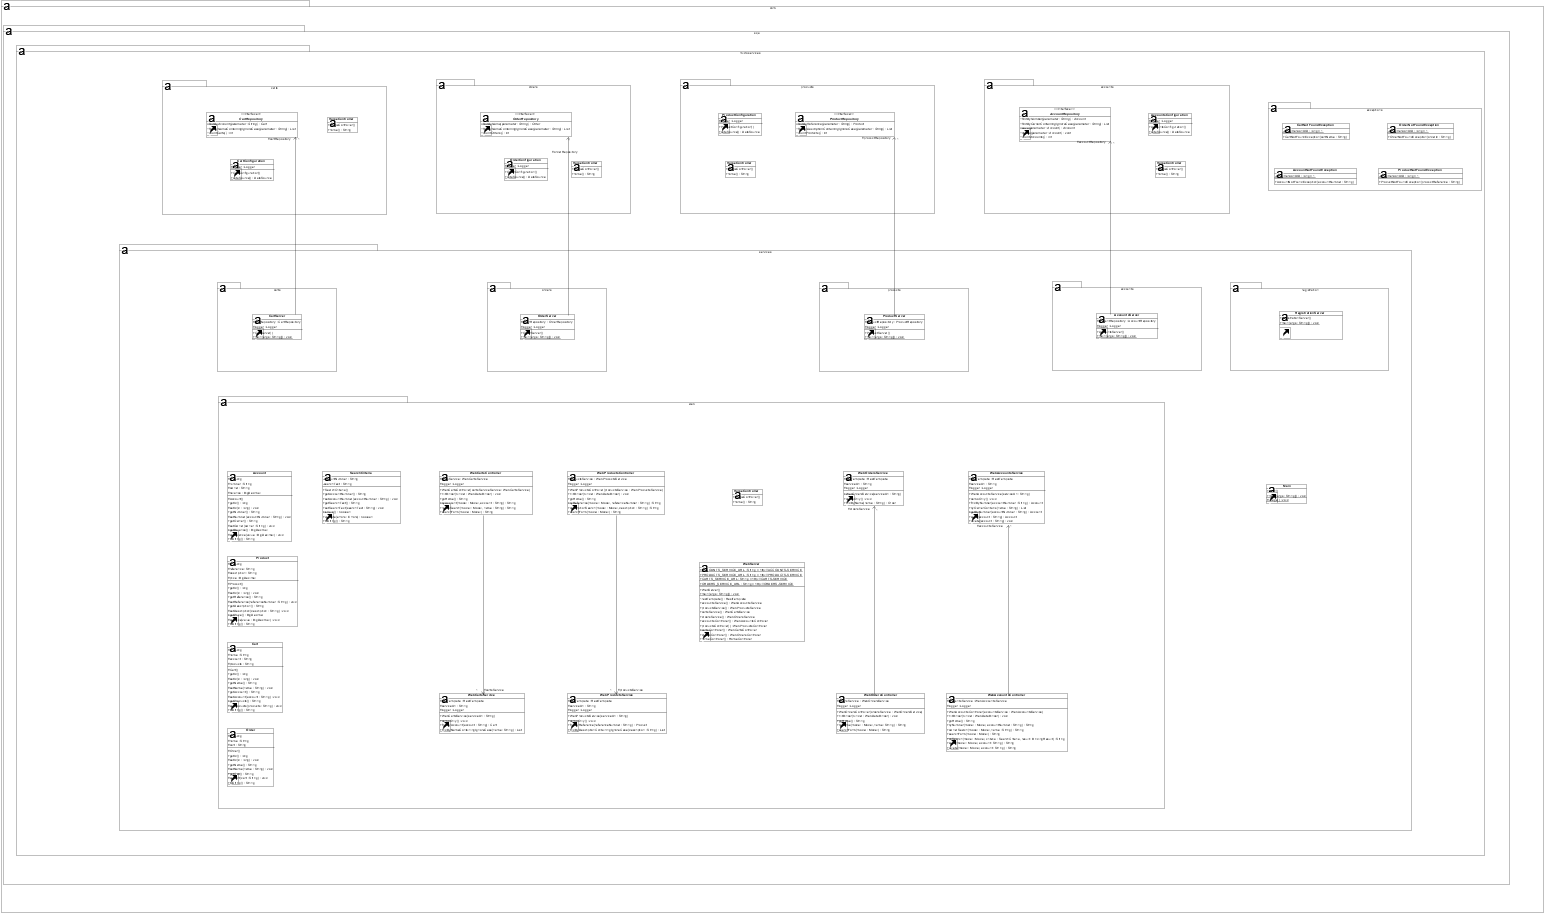
\includegraphics[width=\textwidth,height=\textheight,keepaspectratio]{Figures/ClassDiagram.png}
\decoRule
\caption[Class Diagram]{Application class diagram}
\label{fig:Class Diagram}
\end{figure}

\paragraph So at the end the feature files define requirements for both a service provider and a service consumer and that those services shall be independent between each other. In \ref{fig:Class Diagram} the four service packages are found at the top of the diagram (the right most package correspond to the Exceptions classes used by the services) which are Accounts service, Product service, Cart service and Order service. Here is where the data model and the provider REST API is configured. Registration service is configured within Spring and so no need a package here. Each one of these service classes has then a connection to the the server classes below, used for triggering each service and for exposing its REST API. The right most server package host the server class for the Registration service. 

\paragraph Below the server packages for the functional services, there is the Web server package where a consumer REST API for each one of the services is configured and exposed. Finally, the lonely class a the center right of the diagram is the Main class that will call one of the server classes depending on the incoming arguments ([accounts | product | cart | order | web | registration]).

%-----------------------------------------------------------------------------------------------------------------

\section{REST API}

The features described before define some requests to the services that are fulfilled with the following REST API.

\subsection{Producer API}

\subsubsection{Accounts}
\begin{itemize}
	\item \textit{/accounts/{number}}: search for an account by its account number.
	\item \textit{/accounts/owner/{name}}: search for an account by its account owner name.
	\item \textit{/accounts/save/{account}}: saves a new account.
	\item \textit{/accounts/delete/{account}}: deletes an existing account.
\end{itemize}

\subsubsection{Products}
\begin{itemize}
	\item \textit{/products/{reference}}: search for a product by its product reference.
	\item \textit{/products/description/{description}}: search for a product by its product description.
	\item \textit{/products/save/{product}}: saves a new product.
	\item \textit{/products/delete/{product}}: deletes an existing product.
\end{itemize}

\subsubsection{Carts}
\begin{itemize}
	\item \textit{/carts/{account}}: search for a cart by its associated account number.
	\item \textit{/carts/name/{name}}: search for a cart by its name.
	\item \textit{/carts/save/{cart}}: saves a new cart.
	\item \textit{/carts/delete/{cart}}: deletes an existing cart.
\end{itemize}

\subsubsection{Orders}
\begin{itemize}
	\item \textit{/orders/{name}}: search for an order by its order name.
	\item \textit{/orders/save/{order}}: saves a new order.
	\item \textit{/orders/delete/{order}}: deletes an existing order.
\end{itemize}


\subsection{Consumer API}

\subsubsection{Web}
Its API is just a mapping to the services consumer API defined below.

\subsubsection{Accounts}
Its API is just a mapping to the Accounts provider API defined above.

\subsubsection{Products}
Its API is just a mapping to the Products provider API defined above.

\subsubsection{Carts}
Its API is just a mapping to the Carts provider API defined above.

\subsubsection{Orders}
Its API is just a mapping to the Orders provider API defined above.

\subsubsection{Registration}
As this service is based in the Eureka project, its API is specified in the corresponding official documentation: 
\hyperref[]{\textcolor[rgb]{0,0,1}{https://github.com/Netflix/eureka/wiki/Eureka-REST-operations}}
Registration service API is not required directly by the features defined in this chapter but is used by the test steps that check connectivity with the Web server and by the ones that verify the availability requirements.


%----------------------------------------------------------------------------------------------------------------- %Test Specification 
% Chapter 4

\chapter{Test Automation} % Main chapter title

\label{Chapter4} % For referencing the chapter elsewhere, use \ref{Chapter1} 

%----------------------------------------------------------------------------------------

% Define some commands to keep the formatting separated from the content 
%\newcommand{\keyword}[1]{\textbf{#1}}
%\newcommand{\tabhead}[1]{\textbf{#1}}
%\newcommand{\code}[1]{\texttt{#1}}
%\newcommand{\file}[1]{\texttt{\bfseries#1}}
%\newcommand{\option}[1]{\texttt{\itshape#1}}

%----------------------------------------------------------------------------------------

\section{Overview}
\paragraph This section explains each part of the Jenkins based pipeline for application building and test automation. As pipelines were an important part in the SQA course, the focus here is more in the jobs that deal with test environment management and test execution. However, a simple job for building the application as well as its dependencies is also implemented.

\paragraph Main difference with the pipelines seen in the course is the use of Docker for deploying the services in the desired test environment. Through a set of configuration files located in the source control repository the services are deployed and the network for connecting each other depending on the test case is configured. The commands that trigger the deployment are executed by the Test Framework before running any set of test cases that need a specific deployment.

\paragraph So besides the mere reason of learning the tool, the use of Docker responds to the necessity of managing test environments automatically so the continuous integration chain is not broken even when running at different test levels.

%----------------------------------------------------------------------------------------

\section{Pipeline}
\paragraph The pipeline consists on 2 jobs:

\begin{itemize}
\item \textit{Build:} compiles the application from a clean Jenkins workspace with Maven and generates the JAR file. It also creates the Docker image from the generated JAR file. Although there are several services, only one JAR is generated and each independent service is run depending on the arguments (check \ref{Chapter2} for reference).

\item \textit{Test:} triggers the Cucumber Runner class targeting the folder where the feature files are. Each feature preconditions will make sure that the correct environment is up and running and each feature post conditions will clean the environment again. So the entire set of features including integration and system levels should be executed without stopping at any time.
\end{itemize}


%----------------------------------------------------------------------------------------

\section{Environment Deployment Approach}
\paragraph The features described in chapter \ref{Chapter3} can be split in three main groups:

\begin{itemize}
\item Integration Level - functional
\item System Level - functional
\item System Level - non functional
\end{itemize}

\paragraph The features within the Integration group would only need three services running at the same time as a prerequisite (Web service, Registration service and the service under test) while the features within the System Level group would need all the services to be up and running as the System Level wants to test end to end test cases and besides to look for unknown dependencies or collisions between the services deployed even if they are independent from each other.

 %Test Execution Automation
% Chapter 5

\chapter{Project Planning And Work Achieved} % Main chapter title

\label{Chapter5} % For referencing the chapter elsewhere, use \ref{Chapter1} 

%----------------------------------------------------------------------------------------

% Define some commands to keep the formatting separated from the content 
%\newcommand{\keyword}[1]{\textbf{#1}}
%\newcommand{\tabhead}[1]{\textbf{#1}}
%\newcommand{\code}[1]{\texttt{#1}}
%\newcommand{\file}[1]{\texttt{\bfseries#1}}
%\newcommand{\option}[1]{\texttt{\itshape#1}}

%----------------------------------------------------------------------------------------

\section{Project Planning}

\paragraph At the beginning of the project, a planning was requested with the main tasks to be done and the estimated efforts for each one. Table \ref{tab:planning} shows this planning as well as the actual effort needed for each task.

\begin{table}[htbp]
	\centering
		\begin{tabular}{| m{7em} | m{7cm}| m{2cm} | m{1cm} |} 
		 \hline
		 \textbf{Task}            & \textbf{Description}                                    & \textbf{Estimation} & \textbf{Actual} \\
		 \hline
		 Application Development  & Coding of the application, including learning Spring FW & 5h                  & 15h \\ 
		 \hline
		 Features Definition      & Writing of the features in Gherkin format               & 5h                  & 5h  \\ 
		 \hline
		 Test Step Implementation & Coding of the test steps until they all pass            & 20h                 & 10h \\
		 \hline
		 Pipeline: Docker         & Docker learning, creation of the images and coding      & 20h                 & 15h \\
		 \hline
		 Pipeline: Other jobs     & Maven build and test jobs (only triggering)             & 5h                  & 5h \\
		 \hline
		 Report                   & This document                                           & 5h                  & 10h \\ [1ex] 
		 \hline
		\end{tabular}
	\caption{Planning and Efforts}
	\label{tab:planning}
\end{table}

\paragraph More or less same total amount of hours expected than dedicated
%----------------------------------------------------------------------------------------

\section{Work Achieved}


 %Descripción del trabajo realizado (estructura propia); Planificación final
% Chapter 6

\chapter{Conclusions, Solved Problems and Difficulties} % Main chapter title

\label{Chapter6} % For referencing the chapter elsewhere, use \ref{Chapter1} 

%----------------------------------------------------------------------------------------

% Define some commands to keep the formatting separated from the content 
%\newcommand{\keyword}[1]{\textbf{#1}}
%\newcommand{\tabhead}[1]{\textbf{#1}}
%\newcommand{\code}[1]{\texttt{#1}}
%\newcommand{\file}[1]{\texttt{\bfseries#1}}
%\newcommand{\option}[1]{\texttt{\itshape#1}}

%----------------------------------------------------------------------------------------

\section{Difficulties And Solved Problems}

\subsection{Docker}
\paragraph The use of Docker has been a challenge since the very beginning as it was never used by the author before. There was an initial  knowledge gathering period before deciding which ones of the three main tools released under the Docker umbrella (Docker Engine, Compose and Swarm) needed to be used to meet the project requirements.

\paragraph The initial approach was to use Docker Engine for creating containers from each one of the services and afterward to use Compose for deploying sets of services with one single command. This is particularly useful for deploying complex integration environments with several services and specific network configurations. However, the application built was so simple that using Compose would have made things more complex than what actually are. Moreover, the development environment configured for developing the application consists on one single project and thus one single executable file making impossible to create different container images and so a coherent Compose file. For these reasons the final approach consists only on using Engine for creating containers of the services and running them with the commands provided by Engine.

\paragraph As Docker is a native application for Linux systems, it was used a Linux based laptop for investigating about Docker and its flavors as well as for the initial application development. However, this machine quickly went out of hardware resources when running the six services of the application, the test execution and the Jenkins machine at the same time. For this reason, the author had to change to a laptop with increased resources but based on Windows 7. The drawback of this is that Docker will not run directly on Windows systems below version 10 and thus a solution based on Linux virtual machines shall be used instead in order to overcome this problem but at the same time this created more problems due to the certificate paths for SSH connections already set up in that machine.
At the end some workarounds were applied and the system was able to work but leaving clear that the native versions of Docker should be used for productive environments. 


\subsection{Spring Framework}

\paragraph Using Spring development framework for the application was actually a try for using the need of having to develop something for learning a new technology used widely these days. As the Accounts service was half developed as the content of a Spring-based demo, the idea was to keep expanding the application with the other services using Spring taking as a reference code written in the demo. This soon showed up as a bad idea from the timing perspective as learning the basics of Spring took more time than expected and do not provide any additional functionality that could not be implemented with traditional server-client libraries.

\paragraph Another unexpected drawback of using Spring is the amount of resources that consumes for one single service. While this is the price to pay for being so simple to code, it provided no benefit due to the limited scope of the application.


\subsection{Cucumber}

\paragraph While writing test steps for the Gherkin files is relatively easy, the challenge comes when several different test targets need more or less the same test functionality and thus a way of generalizing steps has to be found. In this case this generalization is done in the form of one class per service acting as a client extending a base client class with shared methods and abstract classes that creates the requests to be sent to the system. Then, in the step, only one line calls to these clients are written easing this way the maintenance of the test step library by reducing to a minimum the source code. When this is done, adding new feature files becomes a straightforward activity.

\paragraph Conclusion here would be that in order to assure a controlled growing of the test step library, is better to use more test steps  with less logic inside rather than less in number but bigger test steps. While is true that the test step library becomes larger this way, it could be easily sorted (i.e. alphabetically) and reviewed.

\paragraph As soon as the test developer starts increasing the functionality done by the classes in the background, some usual coding issues appear and thus is important to apply coding conventions here as well. More relevant example due to the testing focus of the code (test steps in this case) being developed is exception handling. By default, any test step will throw "`Throwable"' super class which essentially means that any Error or Exception raised by the code will be considered an actual error and the step will exit with error code 1. While this approach is fine from the test run point of view, the developer should make sure that the background test classes and the source code under test handle exceptions properly so the output of the test step can provide useful information about the error.
 

\section{Conclusions}

\paragraph The implementation of the solution proposed in this document did not happen without unexpected issues and problems of several kinds. However, the author finds the experience enriching in the sense that the project objectives accomplished indeed provided knowledge and an overall idea of the technologies used for the solution which in fact was the main objective in the background.

\paragraph Having to overcome different problems is also part of the experience although viewed in retrospective some project objectives like using Spring could have been skipped as it did not provide additional value to the project and made the application development harder than the strictly necessary being a subject not included in the course agenda. 




 %Conclusions;


%----------------------------------------------------------------------------------------
%	THESIS CONTENT - APPENDICES
%----------------------------------------------------------------------------------------

%\appendix % Cue to tell LaTeX that the following "chapters" are Appendices

% Include the appendices of the thesis as separate files from the Appendices folder
% Uncomment the lines as you write the Appendices

%% Appendix A

\chapter{Frequently Asked Questions} % Main appendix title

\label{AppendixA} % For referencing this appendix elsewhere, use \ref{AppendixA}

\section{How do I change the colors of links?}

The color of links can be changed to your liking using:

{\small\verb!\hypersetup{urlcolor=red}!}, or

{\small\verb!\hypersetup{citecolor=green}!}, or

{\small\verb!\hypersetup{allcolor=blue}!}.

\noindent If you want to completely hide the links, you can use:

{\small\verb!\hypersetup{allcolors=.}!}, or even better: 

{\small\verb!\hypersetup{hidelinks}!}.

\noindent If you want to have obvious links in the PDF but not the printed text, use:

{\small\verb!\hypersetup{colorlinks=false}!}.

%\include{Appendices/AppendixB}
%\include{Appendices/AppendixC}

%----------------------------------------------------------------------------------------
%	BIBLIOGRAPHY
%----------------------------------------------------------------------------------------

\printbibliography[heading=bibintoc]

%----------------------------------------------------------------------------------------

\end{document}  
